\documentclass[aspectratio=169, 10pt]{beamer}
\usetheme{metropolis}
% \usefonttheme{professionalfonts}

\usepackage[english]{babel}
\usepackage[style=authortitle,backend=biber]{biblatex}
\usepackage[utf8]{inputenc}
\usepackage{algorithmic}
\usepackage{amsfonts}
\usepackage{amsmath}
\usepackage{amssymb}
\usepackage{array}
\usepackage{booktabs}
\usepackage{caption}
\usepackage{colortbl}
\usepackage{csquotes}
\usepackage{graphicx}
\usepackage{heuristica}
\usepackage{hyperref}
\usepackage{mathptmx}
\usepackage{multirow}
\usepackage{pgfplots}
\usepackage{siunitx}
\usepackage{subcaption}
\usepackage{svg}
\usepackage{tabularx}
\usepackage{textcomp}
\usepackage{xcolor}
\usepackage{bm}

\addbibresource{references.bib}

\usetikzlibrary{calc}

% \pgfplotsset{compat=1.17}
\usepgfplotslibrary{statistics}

\definecolor{uniblue}{HTML}{00467f}
\definecolor{uniblueDark}{HTML}{002052}
\definecolor{uniblueLight}{HTML}{4671af}
\definecolor{blueGrey}{HTML}{cfd8dc}
\definecolor{red800Dark}{HTML}{8e0000}
\definecolor{green800Dark}{HTML}{005005}

\setbeamercolor{background canvas}{bg=white}
% \setbeamertemplate{frame footer}{\insertshortauthor}
\setbeamerfont{page number in head/foot}{size=\tiny}
% \setbeamercolor{footline}{fg=white, bg=uniblue}
\setbeamercolor{footline}{fg=uniblue}
\setbeamercolor{title}{fg=uniblueDark, bg=white}
\setbeamercolor{frametitle}{fg=white, bg=uniblue}
\setbeamercolor{progress bar}{fg=uniblueLight, bg=white}
\setbeamercolor{block title}{use=structure,fg=white,bg=uniblue}
\setbeamercolor{block body}{use=structure,fg=black,bg=blueGrey}
\setbeamercolor{block title alerted}{fg=white,bg=red800Dark}
\setbeamercolor*{block title example}{fg=white, bg=green800Dark}
\setbeamercolor{alerted text}{fg=red800Dark}
\setbeamercolor{footnote}{fg=black}
\setbeamertemplate{frametitle continuation}[from second]
\setbeamercolor*{bibliography entry title}{fg=black}
\setbeamercolor*{bibliography entry author}{fg=black}
\setbeamercolor*{bibliography entry location}{fg=black}
\setbeamercolor*{bibliography entry note}{fg=black}
% \setbeamertemplate{bibliography item}{}

\setbeamerfont{author}{size=\normalsize}
\setbeamerfont{institute}{size=\small}
\setbeamerfont{date}{size=\normalsize}

\newcommand{\vect}{\mathbf}

\DeclareMathOperator*{\argmax}{argmax}

\hypersetup{
    colorlinks=false,
    linkcolor=blue,
    filecolor=blue,      
    urlcolor=blue,
}

\title{COMPSCI 762 Tutorial 9}
% \subtitle{Tutorial on Bayesian Networks, kNN, SVM, MDP and Q-Learning}
\subtitle{Tutorial on Reinforcement Learning and Association Rule Mining}
\author{Luke Chang}
\institute{The University of Auckland}
\date{May 2021}


\begin{document}

\frame{\titlepage}

% %-------------------------------------------------------------------------------
\begin{frame}
    \frametitle{Topics}

    \tableofcontents
        
\end{frame}

%-------------------------------------------------------------------------------
\section{Reinforcement Learning}
\begin{frame}[t]
\frametitle{Terminology}

\begin{itemize}
    \item \textbf{Agent:} A hypothetical entity which performs actions in an environment to gain some reward.
    \item \textbf{Environment:} A scenario the agent has to face.
    \item \textbf{Action $a_t \in A$:} All the possible moves that the agent can take.
    \item \textbf{State $s_t \in S$:} Current situation returned by the environment.
    \item \textbf{Reward $R(s_t, a_t)$:} An immediate return sent back from the environment to evaluate the last action by the agent.
    \item \textbf{Policy $\pi: S \to A$:} The strategy that the agent employs to determine next action based on the current state.
    \item \textbf{Value $V^\pi(s)$:} The expected long-term return with discount $\gamma$, as opposed to the short term reward $R$. 
        $V^\pi(s)$ is defined as the expected long term return of the current state $s$ under policy $\pi$.
    \item \textbf{Q-value, action-value $Q^\pi(s, a)$:} is similar to \textbf{Value}, except it takes the current action $a$.
        $Q^\pi(s, a)$ refers to the long term return of the current state $s$, taking action $a$ under policy $\pi$.
\end{itemize}


\end{frame}

%-------------------------------------------------------------------------------
\begin{frame}[t]
\frametitle{Markov Decision Process (MDP)}
MDP is defined by $(S, A, R, \mathbb{P}, \gamma)$
\begin{itemize}
    \item $S$: Set of possible states $s_t \in S$
    \item $A$: Set of possible actions $a_t \in A$
    \item $R$: Immediate reward given by the state and action pair $R(s_t, a_t)$
    \item $\mathbb{P}$: Transition probability at state $s$ if an action $a$ is taken
    \item $\gamma$: Discount factor with $0 \leq \gamma < 1$; The weight of future rewards
\end{itemize}

\textbf{Markov Property:} 
\[
    P(s_{t+1}|s_t, a_t, s_{t-1}, a_{t-1}, s_{t-2}, a_{t-2}, \ldots) = P(s_{t+1}|s_t, a_t)
\]

A \textit{stochastic process}, where the future is solely determined by the current state and action. The past and the future are independent.

\end{frame}

%-------------------------------------------------------------------------------
\begin{frame}[t]
\frametitle{Markov Decision Process}

\begin{itemize}
    \item Assume the reward $r_t$ the Markov property:
    \[
        P(r_t|<s_t, a_t>, <s_{t-1}, a_{t-1}>, <s_{t-2}, a_{t-2}>, \ldots) = P(r_t|s_t, a_t)
    \]
    Immediate reward $r_t$ is solely based on the current state and action pair $R(s_t, a_t)$.
    \item \textbf{The task:} Learn a policy $\pi: S \to A$ to maximizes the expected current and future rewards
    \[
        \mathbb{E}[r_t + \gamma r_{t+1} + \gamma^2 r_{t+2} + \ldots]
    \]
    for every possible starting state $s_0$.
    \item \textbf{Intuition:} How we got here doesn’t matter, what is the current best move?
\end{itemize}

\end{frame}

%-------------------------------------------------------------------------------
\begin{frame}[t]
\frametitle{Escape the grid-world: Solving an MDP - Value Iteration}

Your task is to design the AI to help a robot to escape the room. The door is at right top corner. The actions are $\{ \text{Left}, \text{Up}, \text{Right}, \text{Down}\}$.

\begin{figure}
    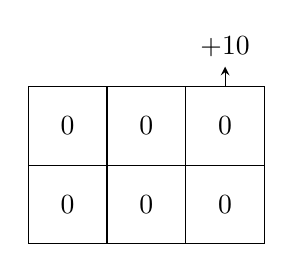
\begin{tikzpicture}
        \draw[step=1cm,color=black] (0, 0) grid (3, 2);
        \node at (2.5, 2.5) {+10};

        \node at (0.5, 0.5) {0};
        \node at (1.5, 0.5) {0};
        \node at (2.5, 0.5) {0};

        \node at (0.5, 1.5) {0};
        \node at (1.5, 1.5) {0};
        \node at (2.5, 1.5) {0};
        
        \draw [-stealth](2.5, 2) -- (2.5, 2.25);
    \end{tikzpicture}
\end{figure}

Initially, no action is taken, we set the value to 0 for all states.
\end{frame}

%-------------------------------------------------------------------------------
\begin{frame}[t]
    \frametitle{Value Iteration - 1 Action}
    
    If we can only take 1 action in the game.

    \begin{figure}
        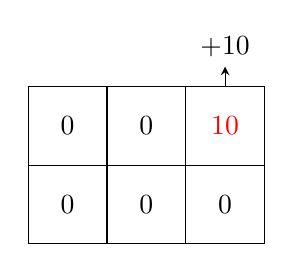
\begin{tikzpicture}
            \draw[step=1cm,color=black] (0, 0) grid (3, 2);
            \node at (2.5, 2.5) {+10};
    
            \node at (0.5, 0.5) {0};
            \node at (1.5, 0.5) {0};
            \node at (2.5, 0.5) {0};
    
            \node at (0.5, 1.5) {0};
            \node at (1.5, 1.5) {0};
            \node at (2.5, 1.5) {\textcolor{red}{10}};
            
            \draw [-stealth](2.5, 2) -- (2.5, 2.25);
        \end{tikzpicture}
    \end{figure}
    
\end{frame}

%-------------------------------------------------------------------------------
\begin{frame}[t]
    \frametitle{Value Iteration - 2 Actions}
    
    When we take more than one action, we have to balance immediate reward and future reward.
    $\gamma$ controls the importance of future rewards.

    \vspace{1em}
    Let $\gamma = 0.5$, state values with 2 actions:

    \begin{equation*}
        \begin{array} {rcl}
            V^\pi(s) & =  \mathbb{E}[\sum_{t \geq 0} \gamma ^t r_t] = r_0 + \gamma r_{1} + \gamma^2 r_{2} + \ldots \\
                     & =  0 + 0.5 \times 10 = 5
        \end{array}
    \end{equation*}

    \begin{figure}
        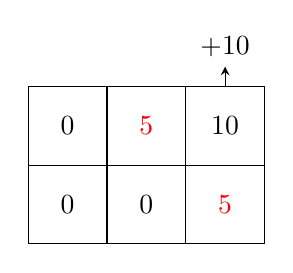
\begin{tikzpicture}
            \draw[step=1cm,color=black] (0, 0) grid (3, 2);
            \node at (2.5, 2.5) {+10};
    
            \node at (0.5, 0.5) {0};
            \node at (1.5, 0.5) {0};
            \node at (2.5, 0.5) {\textcolor{red}{5}};
    
            \node at (0.5, 1.5) {0};
            \node at (1.5, 1.5) {\textcolor{red}{5}};
            \node at (2.5, 1.5) {10};
            
            \draw [-stealth](2.5, 2) -- (2.5, 2.25);
        \end{tikzpicture}
    \end{figure}

\end{frame}

%-------------------------------------------------------------------------------
\begin{frame}[t]
    \frametitle{Value Iteration - 3 Actions}

    Let $\gamma = 0.5$, state values with 3 actions:

    \begin{equation*}
            V^\pi(s) = 0 + 0 + 0.5^2 \times 10 = 2.5
    \end{equation*}

    \begin{figure}
        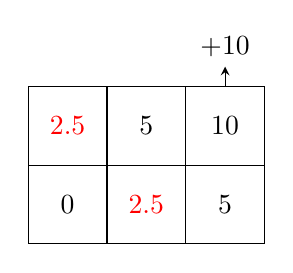
\begin{tikzpicture}
            \draw[step=1cm,color=black] (0, 0) grid (3, 2);
            \node at (2.5, 2.5) {+10};
    
            \node at (0.5, 0.5) {0};
            \node at (1.5, 0.5) {\textcolor{red}{2.5}};
            \node at (2.5, 0.5) {5};
    
            \node at (0.5, 1.5) {\textcolor{red}{2.5}};
            \node at (1.5, 1.5) {5};
            \node at (2.5, 1.5) {10};
            
            \draw [-stealth](2.5, 2) -- (2.5, 2.25);
        \end{tikzpicture}
    \end{figure}

\end{frame}

%-------------------------------------------------------------------------------
\begin{frame}[t]
    \frametitle{Value Iteration}

    Let $\gamma = 0.5$, state values with 4 actions:

    \begin{equation*}
            V^\pi(s) = 0 + 0 + 0 + 0.5^3 \times 10 = 1.25
    \end{equation*}

    \begin{figure}
        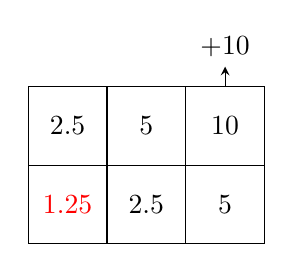
\begin{tikzpicture}
            \draw[step=1cm,color=black] (0, 0) grid (3, 2);
            \node at (2.5, 2.5) {+10};
    
            \node at (0.5, 0.5) {\textcolor{red}{1.25}};
            \node at (1.5, 0.5) {2.5};
            \node at (2.5, 0.5) {5};
    
            \node at (0.5, 1.5) {2.5};
            \node at (1.5, 1.5) {5};
            \node at (2.5, 1.5) {10};
            
            \draw [-stealth](2.5, 2) -- (2.5, 2.25);
        \end{tikzpicture}
    \end{figure}

    \textbf{Caveat:} Do not mix value $V^\pi(s)$ and reward $R(s_t, a_t)$.
\end{frame}


%-------------------------------------------------------------------------------
\begin{frame}[t]
    \frametitle{361 Exam Question 8, 2020}
    
    \begin{example}
        \small
        \begin{itemize}
            \item The black cell cannot be entered.
            % \item For the transitions into non-existing cell the next state, $s'$, is equal to the current state, $s$.
            \item The actions are $\{ \text{Left}, \text{Up}, \text{Right}, \text{Down}\}$.
            % \item For each action, the agent gets a reward of $-1$. The reward for actions that bring it into the target is $0$, and the black state is $-2$.
            \item The reward for actions that bring it into the target is $0$. Other actions get a reward of $-1$.
            \item The partial policy, $\pi$, is given by the arrows in the grid. 
            \item Discount factor, $\gamma = 0.5$
        \end{itemize}
    
        \begin{figure}
            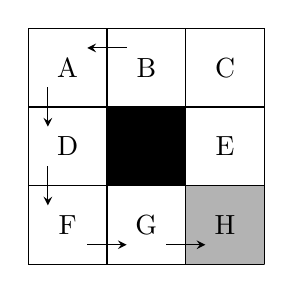
\begin{tikzpicture}
                \draw[step=1cm,color=black] (0, 0) grid (3, 3);
                \node[rectangle,draw,fill = black,minimum width = 1cm,minimum height = 1cm] at (1.5, 1.5) {};
                \node[rectangle,draw,fill = gray,opacity = 0.6,minimum width = 1cm,minimum height = 1cm] at (2.5, 0.5) {};
        
                \node at (0.5, 0.5) {F};
                \node at (1.5, 0.5) {G};
                \node at (2.5, 0.5) {H};
        
                \node at (0.5, 1.5) {D};
                \node at (1.5, 1.5) {};
                \node at (2.5, 1.5) {E};
                
                \node at (0.5, 2.5) {A};
                \node at (1.5, 2.5) {B};
                \node at (2.5, 2.5) {C};
    
                \draw [-stealth](1.25, 2.75) -- (0.75, 2.75);
                \draw [-stealth](0.25, 2.25) -- (0.25, 1.75);
                \draw [-stealth](0.25, 1.25) -- (0.25, 0.75);
                \draw [-stealth](0.75, 0.25) -- (1.25, 0.25);
                \draw [-stealth](1.75, 0.25) -- (2.25, 0.25);
            \end{tikzpicture}
        \end{figure}
    \end{example}

\end{frame}

%-------------------------------------------------------------------------------
\begin{frame}[t]
    \frametitle{361 Exam Question 8, 2020}
    \small

    \begin{itemize}
        % \item The black cell cannot be entered.
        % \item For the transitions into non-existing cell the next state, $s'$, is equal to the current state, $s$.
        % \item The actions are $\{ \text{Left}, \text{Up}, \text{Right}, \text{Down}\}$.
        % \item For each action, the agent gets a reward of $-1$. The reward for actions that bring it into the target is $0$, and the black state is $-2$.
        \item The reward for actions that bring it into the target is $0$. Other actions get a reward of $-1$.
        \item The partial policy, $\pi$, is given by the arrows in the grid. 
        \item $\gamma = 0.5$
    \end{itemize}

    Give for each state the value of the value function, $V$, for the given policy. 
    You can ignore states for which no policy is defined.

    \begin{figure}
        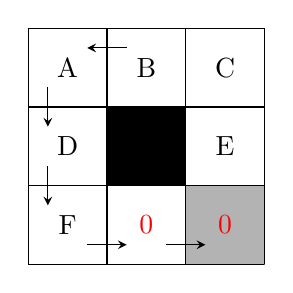
\begin{tikzpicture}
            \draw[step=1cm,color=black] (0, 0) grid (3, 3);
            \node[rectangle,draw,fill = black,minimum width = 1cm,minimum height = 1cm] at (1.5, 1.5) {};
            \node[rectangle,draw,fill = gray,opacity = 0.6,minimum width = 1cm,minimum height = 1cm] at (2.5, 0.5) {};
    
            \node at (0.5, 0.5) {F};
            \node at (1.5, 0.5) {\textcolor{red}{0}};
            \node at (2.5, 0.5) {\textcolor{red}{0}};
    
            \node at (0.5, 1.5) {D};
            \node at (1.5, 1.5) {};
            \node at (2.5, 1.5) {E};
            
            \node at (0.5, 2.5) {A};
            \node at (1.5, 2.5) {B};
            \node at (2.5, 2.5) {C};

            \draw [-stealth](1.25, 2.75) -- (0.75, 2.75);
            \draw [-stealth](0.25, 2.25) -- (0.25, 1.75);
            \draw [-stealth](0.25, 1.25) -- (0.25, 0.75);
            \draw [-stealth](0.75, 0.25) -- (1.25, 0.25);
            \draw [-stealth](1.75, 0.25) -- (2.25, 0.25);
        \end{tikzpicture}
    \end{figure}

    \begin{itemize}
        \item The target state, H, requires 0 action, $V^\pi(s=H) = 0$. Note: There is no action called ``stay''.
        \item State G requires 1 action, $V^\pi(s=G) = 0$
    \end{itemize}
\end{frame}

%-------------------------------------------------------------------------------
\begin{frame}[t]
    \frametitle{361 Exam Question 8, 2020}
    \small

    \begin{itemize}
        % \item The black cell cannot be entered.
        % \item For the transitions into non-existing cell the next state, $s'$, is equal to the current state, $s$.
        % \item The actions are $\{ \text{Left}, \text{Up}, \text{Right}, \text{Down}\}$.
        % \item For each action, the agent gets a reward of $-1$. The reward for actions that bring it into the target is $0$, and the black state is $-2$.
        \item The reward for actions that bring it into the target is $0$. Other actions get a reward of $-1$.
        \item The partial policy, $\pi$, is given by the arrows in the grid. 
        \item $\gamma = 0.5$
    \end{itemize}

    \begin{figure}
        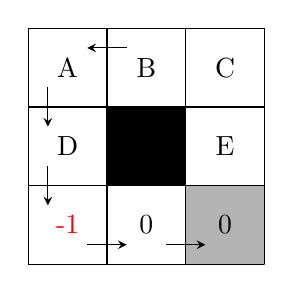
\begin{tikzpicture}
            \draw[step=1cm,color=black] (0, 0) grid (3, 3);
            \node[rectangle,draw,fill = black,minimum width = 1cm,minimum height = 1cm] at (1.5, 1.5) {};
            \node[rectangle,draw,fill = gray,opacity = 0.6,minimum width = 1cm,minimum height = 1cm] at (2.5, 0.5) {};
    
            \node at (0.5, 0.5) {\textcolor{red}{-1}};
            \node at (1.5, 0.5) {0};
            \node at (2.5, 0.5) {0};
    
            \node at (0.5, 1.5) {D};
            \node at (1.5, 1.5) {};
            \node at (2.5, 1.5) {E};
            
            \node at (0.5, 2.5) {A};
            \node at (1.5, 2.5) {B};
            \node at (2.5, 2.5) {C};

            \draw [-stealth](1.25, 2.75) -- (0.75, 2.75);
            \draw [-stealth](0.25, 2.25) -- (0.25, 1.75);
            \draw [-stealth](0.25, 1.25) -- (0.25, 0.75);
            \draw [-stealth](0.75, 0.25) -- (1.25, 0.25);
            \draw [-stealth](1.75, 0.25) -- (2.25, 0.25);
        \end{tikzpicture}
    \end{figure}

    \begin{itemize}
        \item State F requires 2 action, $V^\pi(s=F) = -1 + 0.5 \times 0 = -1 $
    \end{itemize}
\end{frame}

%-------------------------------------------------------------------------------
\begin{frame}[t]
    \frametitle{361 Exam Question 8, 2020}
    \small

    \begin{itemize}
        % \item The black cell cannot be entered.
        % \item For the transitions into non-existing cell the next state, $s'$, is equal to the current state, $s$.
        % \item The actions are $\{ \text{Left}, \text{Up}, \text{Right}, \text{Down}\}$.
        % \item For each action, the agent gets a reward of $-1$. The reward for actions that bring it into the target is $0$, and the black state is $-2$.
        \item The reward for actions that bring it into the target is $0$. Other actions get a reward of $-1$.
        \item The partial policy, $\pi$, is given by the arrows in the grid. 
        \item $\gamma = 0.5$
    \end{itemize}

    \begin{figure}
        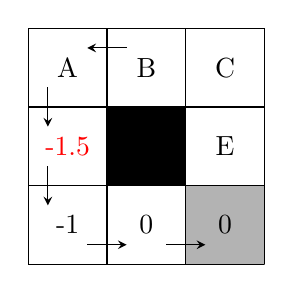
\begin{tikzpicture}
            \draw[step=1cm,color=black] (0, 0) grid (3, 3);
            \node[rectangle,draw,fill = black,minimum width = 1cm,minimum height = 1cm] at (1.5, 1.5) {};
            \node[rectangle,draw,fill = gray,opacity = 0.6,minimum width = 1cm,minimum height = 1cm] at (2.5, 0.5) {};
    
            \node at (0.5, 0.5) {-1};
            \node at (1.5, 0.5) {0};
            \node at (2.5, 0.5) {0};
    
            \node at (0.5, 1.5) {\textcolor{red}{-1.5}};
            \node at (1.5, 1.5) {};
            \node at (2.5, 1.5) {E};
            
            \node at (0.5, 2.5) {A};
            \node at (1.5, 2.5) {B};
            \node at (2.5, 2.5) {C};

            \draw [-stealth](1.25, 2.75) -- (0.75, 2.75);
            \draw [-stealth](0.25, 2.25) -- (0.25, 1.75);
            \draw [-stealth](0.25, 1.25) -- (0.25, 0.75);
            \draw [-stealth](0.75, 0.25) -- (1.25, 0.25);
            \draw [-stealth](1.75, 0.25) -- (2.25, 0.25);
        \end{tikzpicture}
    \end{figure}

    \begin{itemize}
        \item State D requires 3 action, $V^\pi(s=D) = -1 + 0.5 \times (-1) + 0.5^2 \times 0 = -1.5 $
    \end{itemize}
\end{frame}

%-------------------------------------------------------------------------------
\begin{frame}[t]
    \frametitle{361 Exam Question 8, 2020}
    \small

    \begin{itemize}
        % \item The black cell cannot be entered.
        % \item For the transitions into non-existing cell the next state, $s'$, is equal to the current state, $s$.
        % \item The actions are $\{ \text{Left}, \text{Up}, \text{Right}, \text{Down}\}$.
        % \item For each action, the agent gets a reward of $-1$. The reward for actions that bring it into the target is $0$, and the black state is $-2$.
        \item The reward for actions that bring it into the target is $0$. Other actions get a reward of $-1$.
        \item The partial policy, $\pi$, is given by the arrows in the grid. 
        \item $\gamma = 0.5$
    \end{itemize}

    \begin{figure}
        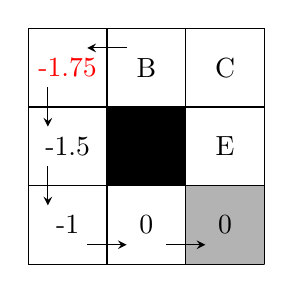
\begin{tikzpicture}
            \draw[step=1cm,color=black] (0, 0) grid (3, 3);
            \node[rectangle,draw,fill = black,minimum width = 1cm,minimum height = 1cm] at (1.5, 1.5) {};
            \node[rectangle,draw,fill = gray,opacity = 0.6,minimum width = 1cm,minimum height = 1cm] at (2.5, 0.5) {};
    
            \node at (0.5, 0.5) {-1};
            \node at (1.5, 0.5) {0};
            \node at (2.5, 0.5) {0};
    
            \node at (0.5, 1.5) {-1.5};
            \node at (1.5, 1.5) {};
            \node at (2.5, 1.5) {E};
            
            \node at (0.5, 2.5) {\textcolor{red}{-1.75}};
            \node at (1.5, 2.5) {B};
            \node at (2.5, 2.5) {C};

            \draw [-stealth](1.25, 2.75) -- (0.75, 2.75);
            \draw [-stealth](0.25, 2.25) -- (0.25, 1.75);
            \draw [-stealth](0.25, 1.25) -- (0.25, 0.75);
            \draw [-stealth](0.75, 0.25) -- (1.25, 0.25);
            \draw [-stealth](1.75, 0.25) -- (2.25, 0.25);
        \end{tikzpicture}
    \end{figure}

    \begin{itemize}
        \item State A requires 4 action, $V^\pi(s=A) = -1 + 0.5 \times (-1) + 0.5^2 \times (-1) + 0.5^3 \times 0 = -1.75 $
    \end{itemize}
\end{frame}

%-------------------------------------------------------------------------------
\begin{frame}[t]
    \frametitle{361 Exam Question 8, 2020}
    \small

    \begin{itemize}
        % \item The black cell cannot be entered.
        % \item For the transitions into non-existing cell the next state, $s'$, is equal to the current state, $s$.
        % \item The actions are $\{ \text{Left}, \text{Up}, \text{Right}, \text{Down}\}$.
        % \item For each action, the agent gets a reward of $-1$. The reward for actions that bring it into the target is $0$, and the black state is $-2$.
        \item The reward for actions that bring it into the target is $0$. Other actions get a reward of $-1$.
        \item The partial policy, $\pi$, is given by the arrows in the grid. 
        \item $\gamma = 0.5$
    \end{itemize}

    \begin{figure}
        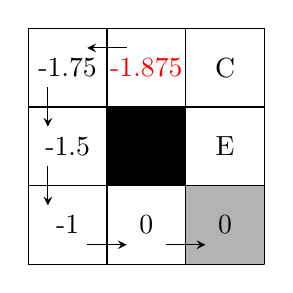
\begin{tikzpicture}
            \draw[step=1cm,color=black] (0, 0) grid (3, 3);
            \node[rectangle,draw,fill = black,minimum width = 1cm,minimum height = 1cm] at (1.5, 1.5) {};
            \node[rectangle,draw,fill = gray,opacity = 0.6,minimum width = 1cm,minimum height = 1cm] at (2.5, 0.5) {};
    
            \node at (0.5, 0.5) {-1};
            \node at (1.5, 0.5) {0};
            \node at (2.5, 0.5) {0};
    
            \node at (0.5, 1.5) {-1.5};
            \node at (1.5, 1.5) {};
            \node at (2.5, 1.5) {E};
            
            \node at (0.5, 2.5) {-1.75};
            \node at (1.5, 2.5) {\textcolor{red}{-1.875}};
            \node at (2.5, 2.5) {C};

            \draw [-stealth](1.25, 2.75) -- (0.75, 2.75);
            \draw [-stealth](0.25, 2.25) -- (0.25, 1.75);
            \draw [-stealth](0.25, 1.25) -- (0.25, 0.75);
            \draw [-stealth](0.75, 0.25) -- (1.25, 0.25);
            \draw [-stealth](1.75, 0.25) -- (2.25, 0.25);
        \end{tikzpicture}
    \end{figure}

    \begin{itemize}
        \item State B requires 5 action, $V^\pi(s=A)=-1+0.5\times (-1)+0.5^2\times (-1)+0.5^3\times (-1)+0.5^4\times 0 = -1.875 $
    \end{itemize}
\end{frame}

%-------------------------------------------------------------------------------
\begin{frame}[t]
\frametitle{Limitations on MDP - The Cliff Sernario}

\begin{itemize}
    \item The value of a state is the expected reward from taking the best action in the state.
    \item Accumulating rewards from random actions would calculate the expected reward from \underline{random actions} in the state.
    \item E.g.: We would learn that any state near a cliff is bad, because you get a negative score if you jump off, even though you don't have to jump off.
\end{itemize}

\begin{figure}
    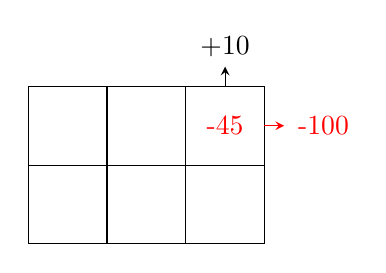
\begin{tikzpicture}
        \draw[step=1cm,color=black] (0, 0) grid (3, 2);
        \node at (2.5, 2.5) {+10};
        \node at (3.75, 1.5) {\textcolor{red}{-100}};

        \node at (0.5, 0.5) {};
        \node at (1.5, 0.5) {};
        \node at (2.5, 0.5) {};

        \node at (0.5, 1.5) {};
        \node at (1.5, 1.5) {};
        \node at (2.5, 1.5) {\textcolor{red}{-45}};
        
        \draw [-stealth](2.5, 2) -- (2.5, 2.25);
        \draw [-stealth,draw=red](3, 1.5) -- (3.25, 1.5);
    \end{tikzpicture}
\end{figure}
    
\end{frame}

%-------------------------------------------------------------------------------
\begin{frame}[t]
\frametitle{Q-Learning}

\textbf{Intuition:} 
Instead of computing value $V^\pi(s)$, we learn \textbf{Q-value}, $Q^\pi(s, a)$, which considers the state $s$ and the action $a$ as a pair.

\begin{itemize}
    \item Q-learning can identify an \textbf{optimal action-selection policy} for any given a finite Markov decision process (FMDP).
    \item $Q: S \times A \to \mathbb{R}$, calculating the quality of a state–action combination
    \item Iterative method, $Q$ is initialized to an arbitrary fixed value. At each time $t$, the agent selects an action $a_t$, observes a reword $r_t$, enters a new state $s_{t+1}$, and $Q$ is updated.
\end{itemize}

\vspace{0.5em}
The Q-value is updated by:

\begin{equation*}
    Q^{\text{new}}(s_t, a_t) \gets Q(s_t, a_t) + \alpha \cdot [R(s_t, a_t) + \gamma \cdot \max_{a'}Q(s_{t+1}, a') - Q(s_t, a_t)]
\end{equation*}

where $\alpha$ is the learning rate. (In a fully deterministic environment, a learning rate of $\alpha = 1$ is optimal.)
\end{frame}

%-------------------------------------------------------------------------------
\begin{frame}[t]
    \frametitle{Q-Learning: 361 Exam Question 8, 2020}
    
    \begin{example}
        \small
        \begin{itemize}
            \item For the transitions into non-existing cell the next state, $s'$, is equal to the current state, $s$.
            \item For each action, the agent gets a reward of $-1$. The reward for actions that bring it into the target is $0$, and the black state is $-2$.
            \item Discount factor, $\gamma = 0.5$
            \item Let the initial value of Q be $-16$.
        \end{itemize}  
        
        \begin{figure}
            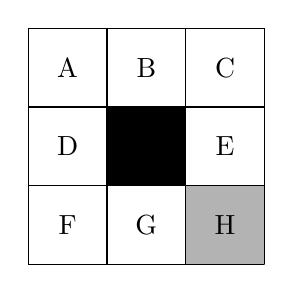
\begin{tikzpicture}
                \draw[step=1cm,color=black] (0, 0) grid (3, 3);
                \node[rectangle,draw,fill = black,minimum width = 1cm,minimum height = 1cm] at (1.5, 1.5) {};
                \node[rectangle,draw,fill = gray,opacity = 0.6,minimum width = 1cm,minimum height = 1cm] at (2.5, 0.5) {};
        
                \node at (0.5, 0.5) {F};
                \node at (1.5, 0.5) {G};
                \node at (2.5, 0.5) {H};
        
                \node at (0.5, 1.5) {D};
                \node at (1.5, 1.5) {};
                \node at (2.5, 1.5) {E};
                
                \node at (0.5, 2.5) {A};
                \node at (1.5, 2.5) {B};
                \node at (2.5, 2.5) {C};
                
            \end{tikzpicture}
        \end{figure}
    \end{example}
    
\end{frame}

%-------------------------------------------------------------------------------
\begin{frame}[t]
    \frametitle{Q-Learning: 361 Exam Question 8, 2020}
    % \small

    Let the agent walks the path (F, right) $\to$ (G, up) $\to$ (G, right). 
    Calculate values for the Q-table after every step of the path.
    What is the value of $V(G)$ after the last step?

    \begin{figure}
        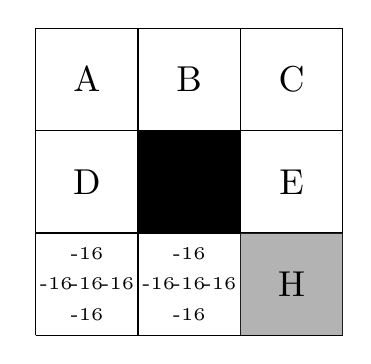
\begin{tikzpicture}[scale=1.3, transform shape]
            \draw[step=1cm,color=black] (0, 0) grid (3, 3);
            \node[rectangle,draw,fill = black,minimum width = 1cm,minimum height = 1cm] at (1.5, 1.5) {};
            \node[rectangle,draw,fill = gray,opacity = 0.6,minimum width = 1cm,minimum height = 1cm] at (2.5, 0.5) {};
    
            % \node at (0.5, 0.5) {F};
            % \node at (1.5, 0.5) {G};
            \node at (2.5, 0.5) {H};
    
            \node at (0.5, 1.5) {D};
            \node at (1.5, 1.5) {};
            \node at (2.5, 1.5) {E};
            
            \node at (0.5, 2.5) {A};
            \node at (1.5, 2.5) {B};
            \node at (2.5, 2.5) {C};

            \node[font=\tiny] at (1.5, 0.5) {-16};
            \node[font=\tiny] at (1.5, 0.8) {-16};
            \node[font=\tiny] at (1.5, 0.2) {-16};
            \node[font=\tiny] at (1.2, 0.5) {-16};
            \node[font=\tiny] at (1.8, 0.5) {-16};

            \node[font=\tiny] at (0.5, 0.5) {-16};
            \node[font=\tiny] at (0.5, 0.8) {-16};
            \node[font=\tiny] at (0.5, 0.2) {-16};
            \node[font=\tiny] at (0.2, 0.5) {-16};
            \node[font=\tiny] at (0.8, 0.5) {-16};
    
            % \draw [-stealth](1.5, 2.75) -- (0.75, 2.75);
            % \draw [-stealth](0.25, 2.5) -- (0.25, 1.75);
            % \draw [-stealth](0.25, 1.5) -- (0.25, 0.75);
            % \draw [-stealth](0.75, 0.25) -- (1.25, 0.25);
            % \draw [-stealth](1.5, 0.25) -- (2.25, 0.25);
            
        \end{tikzpicture}
    \end{figure}
    
\end{frame}

%-------------------------------------------------------------------------------
\begin{frame}[t]
    \frametitle{Q-Learning: 361 Exam Question 8, 2020}
    % \small
    
    Let the agent walks the path (F, right) $\to$ (G, up) $\to$ (G, right). 
    Calculate values for the Q-table after every step of the path.
    What is the value of $V(G)$ after the last step?

    \begin{figure}
        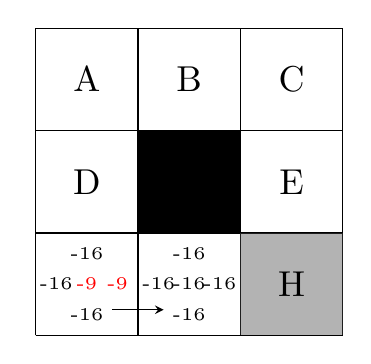
\begin{tikzpicture}[scale=1.3, transform shape]
            \draw[step=1cm,color=black] (0, 0) grid (3, 3);
            \node[rectangle,draw,fill = black,minimum width = 1cm,minimum height = 1cm] at (1.5, 1.5) {};
            \node[rectangle,draw,fill = gray,opacity = 0.6,minimum width = 1cm,minimum height = 1cm] at (2.5, 0.5) {};

            \node at (2.5, 0.5) {H};
    
            \node at (0.5, 1.5) {D};
            \node at (1.5, 1.5) {};
            \node at (2.5, 1.5) {E};
            
            \node at (0.5, 2.5) {A};
            \node at (1.5, 2.5) {B};
            \node at (2.5, 2.5) {C};

            \node[font=\tiny] at (1.5, 0.5) {-16};
            \node[font=\tiny] at (1.5, 0.8) {-16};
            \node[font=\tiny] at (1.5, 0.2) {-16};
            \node[font=\tiny] at (1.2, 0.5) {-16};
            \node[font=\tiny] at (1.8, 0.5) {-16};

            \node[font=\tiny] at (0.5, 0.5) {\textcolor{red}{-9}};
            \node[font=\tiny] at (0.5, 0.8) {-16};
            \node[font=\tiny] at (0.5, 0.2) {-16};
            \node[font=\tiny] at (0.2, 0.5) {-16};
            \node[font=\tiny] at (0.8, 0.5) {\textcolor{red}{-9}};
    
            \draw [-stealth](0.75, 0.25) -- (1.25, 0.25);
        \end{tikzpicture}
    \end{figure}
    
    Given $\gamma = 0.5$, $Q(s=F, a=\text{right}) = -1 + 0.5 \times (-16) = -9$
\end{frame}

%-------------------------------------------------------------------------------
\begin{frame}[t]
    \frametitle{Q-Learning: 361 Exam Question 8, 2020}
    % \small
    
    Let the agent walks the path (F, right) $\to$ (G, up) $\to$ (G, right). 
    Calculate values for the Q-table after every step of the path.
    What is the value of $V(G)$ after the last step?

    \begin{figure}
        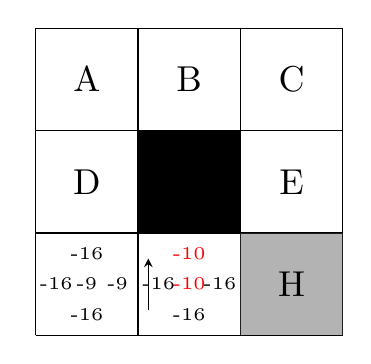
\begin{tikzpicture}[scale=1.3, transform shape]
            \draw[step=1cm,color=black] (0, 0) grid (3, 3);
            \node[rectangle,draw,fill = black,minimum width = 1cm,minimum height = 1cm] at (1.5, 1.5) {};
            \node[rectangle,draw,fill = gray,opacity = 0.6,minimum width = 1cm,minimum height = 1cm] at (2.5, 0.5) {};
    
            % \node at (0.5, 0.5) {F};
            % \node at (1.5, 0.5) {G};
            \node at (2.5, 0.5) {H};
    
            \node at (0.5, 1.5) {D};
            \node at (1.5, 1.5) {};
            \node at (2.5, 1.5) {E};
            
            \node at (0.5, 2.5) {A};
            \node at (1.5, 2.5) {B};
            \node at (2.5, 2.5) {C};

            \node[font=\tiny] at (1.5, 0.5) {\textcolor{red}{-10}};
            \node[font=\tiny] at (1.5, 0.8) {\textcolor{red}{-10}};
            \node[font=\tiny] at (1.5, 0.2) {-16};
            \node[font=\tiny] at (1.2, 0.5) {-16};
            \node[font=\tiny] at (1.8, 0.5) {-16};

            \node[font=\tiny] at (0.5, 0.5) {-9};
            \node[font=\tiny] at (0.5, 0.8) {-16};
            \node[font=\tiny] at (0.5, 0.2) {-16};
            \node[font=\tiny] at (0.2, 0.5) {-16};
            \node[font=\tiny] at (0.8, 0.5) {-9};
    
            \draw [-stealth](1.1, 0.25) -- (1.1, 0.75);
            
        \end{tikzpicture}
    \end{figure}
    
    \[
        Q(G, \text{up}) = -2 + 0.5 \times (-16) = -10
    \]
\end{frame}

%-------------------------------------------------------------------------------
\begin{frame}[t]
    \frametitle{Q-Learning: 361 Exam Question 8, 2020}
    % \small
    
    Let the agent walks the path (F, right) $\to$ (G, up) $\to$ (G, right). 
    Calculate values for the Q-table after every step of the path.
    What is the value of $V(G)$ after the last step?

    \begin{figure}
        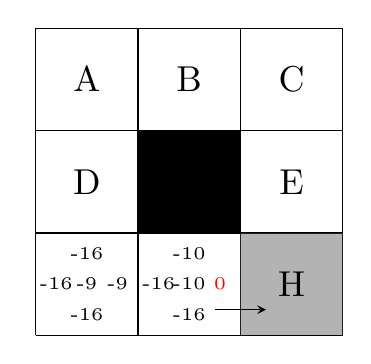
\begin{tikzpicture}[scale=1.3, transform shape]
            \draw[step=1cm,color=black] (0, 0) grid (3, 3);
            \node[rectangle,draw,fill = black,minimum width = 1cm,minimum height = 1cm] at (1.5, 1.5) {};
            \node[rectangle,draw,fill = gray,opacity = 0.6,minimum width = 1cm,minimum height = 1cm] at (2.5, 0.5) {};
    
            % \node at (0.5, 0.5) {F};
            % \node at (1.5, 0.5) {G};
            \node at (2.5, 0.5) {H};
    
            \node at (0.5, 1.5) {D};
            \node at (1.5, 1.5) {};
            \node at (2.5, 1.5) {E};
            
            \node at (0.5, 2.5) {A};
            \node at (1.5, 2.5) {B};
            \node at (2.5, 2.5) {C};

            \node[font=\tiny] at (1.5, 0.5) {-10};
            \node[font=\tiny] at (1.5, 0.8) {-10};
            \node[font=\tiny] at (1.5, 0.2) {-16};
            \node[font=\tiny] at (1.2, 0.5) {-16};
            \node[font=\tiny] at (1.8, 0.5) {\textcolor{red}{0}};

            \node[font=\tiny] at (0.5, 0.5) {-9};
            \node[font=\tiny] at (0.5, 0.8) {-16};
            \node[font=\tiny] at (0.5, 0.2) {-16};
            \node[font=\tiny] at (0.2, 0.5) {-16};
            \node[font=\tiny] at (0.8, 0.5) {-9};
    
            \draw [-stealth](1.75, 0.25) -- (2.25, 0.25);
            
        \end{tikzpicture}
    \end{figure}
    
    \[
        Q(G, \text{right}) = 0 + 0.5 \times 0 = 0
    \]
\end{frame}

%-------------------------------------------------------------------------------
\begin{frame}[t]
    \frametitle{Q-Learning: 361 Exam Question 8, 2020}
    % \small
    
    Let the agent walks the path (F, right) $\to$ (G, up) $\to$ (G, right). 
    Calculate values for the Q-table after every step of the path.
    What is the value of $V(G)$ after the last step?

    \begin{figure}
        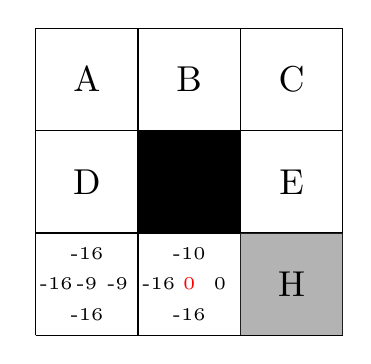
\begin{tikzpicture}[scale=1.3, transform shape]
            \draw[step=1cm,color=black] (0, 0) grid (3, 3);
            \node[rectangle,draw,fill = black,minimum width = 1cm,minimum height = 1cm] at (1.5, 1.5) {};
            \node[rectangle,draw,fill = gray,opacity = 0.6,minimum width = 1cm,minimum height = 1cm] at (2.5, 0.5) {};
    
            % \node at (0.5, 0.5) {F};
            % \node at (1.5, 0.5) {G};
            \node at (2.5, 0.5) {H};
    
            \node at (0.5, 1.5) {D};
            \node at (1.5, 1.5) {};
            \node at (2.5, 1.5) {E};
            
            \node at (0.5, 2.5) {A};
            \node at (1.5, 2.5) {B};
            \node at (2.5, 2.5) {C};

            \node[font=\tiny] at (1.5, 0.5) {\textcolor{red}{0}};
            \node[font=\tiny] at (1.5, 0.8) {-10};
            \node[font=\tiny] at (1.5, 0.2) {-16};
            \node[font=\tiny] at (1.2, 0.5) {-16};
            \node[font=\tiny] at (1.8, 0.5) {0};

            \node[font=\tiny] at (0.5, 0.5) {-9};
            \node[font=\tiny] at (0.5, 0.8) {-16};
            \node[font=\tiny] at (0.5, 0.2) {-16};
            \node[font=\tiny] at (0.2, 0.5) {-16};
            \node[font=\tiny] at (0.8, 0.5) {-9};
    
            % \draw [-stealth](1.75, 0.25) -- (2.25, 0.25);
        \end{tikzpicture}
    \end{figure}
    
    \[ V(G) = 0 \]
\end{frame}

%-------------------------------------------------------------------------------
\begin{frame}[t]
    \frametitle{Q-Learning: 361 Exam Question 8, 2020}
    % \small
    
    Create an optimal policy $\pi^*$, and draw it on the given diagram.
    What are the corresponding values of $V^*$?
    What is the most desirable state for the agent?

    \begin{figure}
        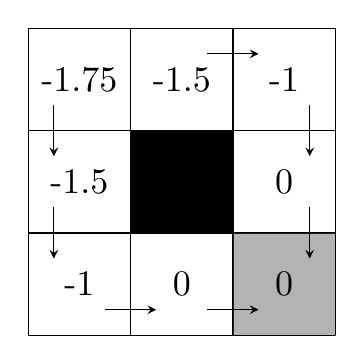
\begin{tikzpicture}[scale=1.3, transform shape]
            \draw[step=1cm,color=black] (0, 0) grid (3, 3);
            \node[rectangle,draw,fill = black,minimum width = 1cm,minimum height = 1cm] at (1.5, 1.5) {};
            \node[rectangle,draw,fill = gray,opacity = 0.6,minimum width = 1cm,minimum height = 1cm] at (2.5, 0.5) {};
    
            \node at (0.5, 0.5) {-1};
            \node at (1.5, 0.5) {0};
            \node at (2.5, 0.5) {0};
    
            \node at (0.5, 1.5) {-1.5};
            \node at (1.5, 1.5) {};
            \node at (2.5, 1.5) {0};
            
            \node at (0.5, 2.5) {-1.75};
            \node at (1.5, 2.5) {-1.5};
            \node at (2.5, 2.5) {-1};
    
            \draw [-stealth](0.25, 2.25) -- (0.25, 1.75);
            \draw [-stealth](0.25, 1.25) -- (0.25, 0.75);
            \draw [-stealth](0.75, 0.25) -- (1.25, 0.25);
            \draw [-stealth](1.75, 0.25) -- (2.25, 0.25);

            \draw [-stealth](1.75, 2.75) -- (2.25, 2.75);
            \draw [-stealth](2.75, 2.25) -- (2.75, 1.75);
            \draw [-stealth](2.75, 1.25) -- (2.75, 0.75);
        \end{tikzpicture}
    \end{figure}
    
    Note: The initial value of $Q$ does not affect $V(s)$.
\end{frame}

%-------------------------------------------------------------------------------
\section{Association Rule Mining}
\begin{frame}[t]
\frametitle{Terminology}
\small

\begin{itemize}
    \item \textbf{Itemset:} A collection of one or more items, e.g. $X = \{A, B\}$, $Y =\{ B \}$ Note: Single item can be an itemset.
    \item \textbf{$\bm{N = |T|}$:} is the number of transactions (instances)
    \item \textbf{$\bm{d = |I|}$:} is the number of distinct (unique) items. There are \textcolor{red}{$2^d$} possible itemsets.
    \item \textbf{Width $\bm{w}$:} The transaction width is the number of items present in a transaction.
    \item \textbf{Support count $\bm{\sigma}$:} Frequency of occurrence of an itemset, e.g. $\sigma(\{A, B\})=2$ means 2 transactions contain the itemset $\{A, B\}$.
    \item \textbf{Frequent Itemset:} An itemset whose support is greater than or equal to the \textcolor{red}{\textit{minsup}} threshold
    \item \textbf{Support $s(X \to Y)$:} Fraction of transactions that contain an itemset
        \[ s(X \to Y) = \frac{\sigma(X \cup Y)}{|T|} \] 
    \item \textbf{Confidence $\bm{c \to Y}$:} Measures how often items in $Y$ appear in transactions that contain $X$
        \[ c(X \to Y) = \frac{\sigma(X \cup Y)}{\sigma(X)} \] 
\end{itemize}


\end{frame}

%-------------------------------------------------------------------------------
\begin{frame}[t]
\frametitle{Apriori Algorithm}

\begin{itemize}
    \item \textbf{Goal:} Reducing the number of candidates
    \item \textbf{Apriori principle:} ``If an itemset is frequent, then all of its subsets must also be frequent.'' -- \textcolor{red}{anti-monotone} property of support
        \[ \forall X, Y:(X \subseteq Y) \Rightarrow s(X) \geq s(Y) \]
    \item \textbf{Maximal Frequent Itemset:} If none of its immediate supersets is frequent
    \item \textbf{Closed Frequent Itemset:} An itemset X is closed, if none of its immediate supersets has the same support as the itemset $X$.
        \[ \text{Maximal Frequent Itemset} \subseteq \text{Closed Frequent Itemset} \subseteq \text{Frequent Itemset} \]
\end{itemize}

\end{frame}

%-------------------------------------------------------------------------------
\begin{frame}[t]
\frametitle{Review Question 1 -- Apriori Algorithms}
\small

Given the following transaction database, considering using Apriori algorithm to find all frequent itemsets a support threshold of 30\%.

\begin{columns}
    \begin{column}{0.5\textwidth} 
        \begin{table}[]
            \begin{tabular}{c|l}
            TID & \textbf{Items}      \\ \hline
            T1   & \textbf{1, 2, 5}    \\
            T2   & \textbf{2, 4}       \\
            T3   & \textbf{2, 3}       \\
            T4   & \textbf{1, 2, 4}    \\
            T5   & \textbf{1, 3}       \\
            T6   & \textbf{2, 3}       \\
            T7   & \textbf{1, 3}       \\
            T8   & \textbf{1, 2, 3, 5} \\
            T9   & \textbf{1, 2, 3}    \\
            T10  & \textbf{1, 2, 5, 6}
            \end{tabular}
        \end{table}
    \end{column}
    \begin{column}{0.5\textwidth} % Right

        \begin{table}[]
            \begin{tabular}{c|c}
                Item                     & Support Count, $\sigma$           \\ \hline
                1                        & 7                        \\
                2                        & 8                        \\
                3                        & 6                        \\
                {\color[HTML]{FE0000} 4} & {\color[HTML]{FE0000} 2} \\
                5                        & 3                        \\
                {\color[HTML]{FE0000} 6} & {\color[HTML]{FE0000} 1}
            \end{tabular}
            \caption{Candidate 1-itemsets}
        \end{table}
        
        \begin{itemize}
            \item 10 transactions. The frequent itemset must occur in at least 3 transactions.
            \item \{1\}, \{2\}, \{3\} and \{5\} are frequent 1-itemsets.
        \end{itemize}
    \end{column}
\end{columns}

\end{frame}

%-------------------------------------------------------------------------------
\begin{frame}[t]
\frametitle{Review Question 1 -- Frequent itemsets}
\small

\begin{columns}
    \begin{column}{0.5\textwidth} 
        \begin{table}[]
            \begin{tabular}{c|c}
                Item                       &  $\sigma$                \\ \hline
                1, 2                       & 7                        \\
                1, 3                       & 4                        \\
                1, 5                       & 3                        \\
                2, 3                       & 4                        \\
                2, 5                       & 3                        \\
                {\color[HTML]{FE0000} 3, 5} & {\color[HTML]{FE0000} 1}
            \end{tabular}
            \caption{Candidate 2-itemsets}
        \end{table}

        \begin{itemize}
            \item $\{3, 5\}$ is not a frequent 2-itemset.
        \end{itemize}
    \end{column}
    \begin{column}{0.5\textwidth} % Right
        \begin{table}[]
            \begin{tabular}{c|c}
                Item                           & $\sigma$            \\ \hline
                {\color[HTML]{FE0000} 1, 2, 3} & {\color[HTML]{FE0000} 2} \\
                1, 2, 5                        & 3                        \\
                {\color[HTML]{FE0000} 1, 3, 5} & {\color[HTML]{FE0000} 1} \\
                {\color[HTML]{FE0000} 2, 3, 5} & {\color[HTML]{FE0000} 1}
            \end{tabular}
            \caption{Candidate 3-itemsets}
        \end{table}

        \begin{itemize}
            \item Only $\{1, 2, 5\}$ is a frequent 3-itemset.
            \item None of 4-itemsets is frequent.
        \end{itemize}
    \end{column}
\end{columns}

\end{frame}

%-------------------------------------------------------------------------------
\begin{frame}[t]
    \frametitle{Review Question 1 -- Confidence Threshold}
    \small

    Find all association rules from frequent 3-itemset with the confidence threshold of 80\%.
    
    \[ c(X \to Y) = \frac{\sigma(X \cup Y)}{\sigma(X)} \] 

    \begin{itemize}
        \item Only $\{1, 2, 5\}$ is a frequent 3-itemset. Remove other 3-itemsets.
        \item $\sigma(X \cup Y) = \sigma (\{ 1, 2, 5\}) = 3$
    \end{itemize}

    \begin{table}[]
        \footnotesize
        \begin{tabular}{c|c|c}
        $X \to Y$                & $\sigma(X)$ & $c(X \to Y)$ \\ \hline
        $\{ 1 \} \to \{  2, 5\}$ & 7           & \textcolor{red}{$3/7 \approx 0.43$} \\ 
        $\{ 2 \} \to \{  1, 5\}$ & 8           & \textcolor{red}{$3/8 = 0.375$} \\ 
        $\{ 5 \} \to \{  1, 2\}$ & 3           & $3/3 = 1$ \\ 
        $\{ 1, 2 \} \to \{  5\}$ & 5           & \textcolor{red}{$3/5 = 0.6$} \\ 
        $\{ 1, 5 \} \to \{  2\}$ & 3           & $3/3 = 1$ \\ 
        $\{ 2, 5 \} \to \{  1\}$ & 3           & $3/3 = 1$ \\ 
        \end{tabular}
    \end{table}

    $\{ 5 \} \to \{  1, 2\}$, $\{ 1, 5 \} \to \{  2\}$ and $\{ 2, 5 \} \to \{  1\}$ are the 3-itemsets, such that $c(X \to Y) \geq \textit{minconf}$ .

\end{frame}

%-------------------------------------------------------------------------------
\begin{frame}[t]
\frametitle{Review Question 2 -- FP-Tree}
\small

Considering the same transactions above, use frequent-pattern (FP) growth algorithm to perform frequent itemsets mining with a support threshold of 30\%.

\begin{enumerate}
    \item What is the item head table? (Hint: keep in mind the support count and sort order.)
    \item What is the FP-tree corresponding to the transactions above?
    % \item What is the conditional pattern base corresponding to the transactions above?
\end{enumerate}

\begin{columns}
    \begin{column}{0.5\textwidth} 
        \begin{table}[]
            \begin{tabular}{c|c|c}
                Item      & $\sigma$  & Node Link \\ \hline
                \textbf{2}         & 8         &           \\
                \textbf{1}         & 7         &           \\
                \textbf{3}         & 6         &           \\
                \textbf{5}         & 3         &           \\
            \end{tabular}
            \caption{Header Table}
        \end{table}

        \textit{Node Links} are omitted. They are pointers which point to the node with the corresponding TID.

    \end{column}
    \begin{column}{0.5\textwidth} % Right
        \begin{figure}
            \center
            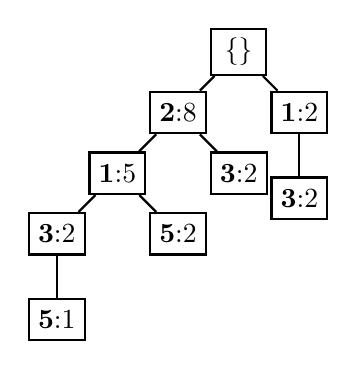
\begin{tikzpicture}[node distance={4em}, thick, main/.style = {draw, node distance=3.1em, rectangle, minimum height=1.5em, minimum width=2em}] 
                \node[main] (1) {\{\}};
                \pause

                \node[main] (2) [below left of=1] {\textbf{2}:8};
                \draw[-] (2) -- (1);
                \pause

                \node[main] (4) [below left of=2] {\textbf{1}:5};
                \draw[-] (4) -- (2);
                \node[main] (3) [below right of=1] {\textbf{1}:2};
                \draw[-] (3) -- (1);
                \pause
                
                \node[main] (5) [below right of=2] {\textbf{3}:2};
                \draw[-] (5) -- (2);
                \node[main] (8) [below left of=4] {\textbf{3}:2};
                \draw[-] (8) -- (4);
                \node[main] (6) [below of=3] {\textbf{3}:2};
                \draw[-] (3) -- (6);
                \pause

                \node[main] (7) [below right of=4] {\textbf{5}:2};
                \draw[-] (7) -- (4);
                \node[main] (9) [below of=8] {\textbf{5}:1};
                \draw[-] (9) -- (8);
            \end{tikzpicture} 
        \end{figure}
    \end{column}
\end{columns}

\end{frame}

\begin{frame}[t]
\frametitle{Review Question 2 -- FP-Tree}
\small

What is the conditional pattern base corresponding to the transactions above?

\begin{columns}
    \begin{column}{0.5\textwidth} 
        \begin{table}[]
            \begin{tabular}{c|c|c}
                Item      & $\sigma$  & Node Link \\ \hline
                \textbf{2}         & 8         &           \\
                \textbf{1}         & 7         &           \\
                \textbf{3}         & 6         &           \\
                \textbf{5}         & 3         &           \\
            \end{tabular}
            \caption{Header Table}
        \end{table}

        \begin{table}[]
            \begin{tabular}{c|l}
                Item      & Conditional Pattern Base \\ \hline
                \textbf{5} & \{(\textbf{1}:2, \textbf{2}:2), (\textbf{3}:1, \textbf{1}:1, \textbf{2}:1) \} \\
                \textbf{3} & \{(\textbf{1}:2, \textbf{2}:2), (\textbf{2}:2), (\textbf{1}:2) \}\\
                \textbf{1} & \{(\textbf{2}:5) \}\\
                \textbf{2} & \{\}\\
            \end{tabular}
        \end{table}
    \end{column}
    \begin{column}{0.5\textwidth} % Right
        \begin{figure}
            \center
            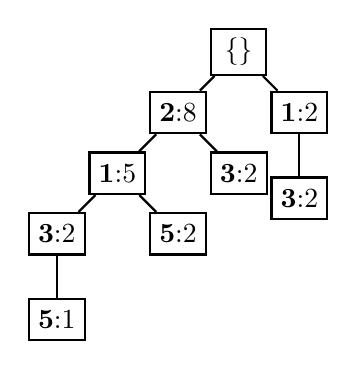
\begin{tikzpicture}[node distance={4em}, thick, main/.style = {draw, node distance=3.1em, rectangle, minimum height=1.5em, minimum width=2em}] 
                \node[main] (1) {\{\}};

                \node[main] (2) [below left of=1] {\textbf{2}:8};
                \draw[-] (2) -- (1);

                \node[main] (4) [below left of=2] {\textbf{1}:5};
                \draw[-] (4) -- (2);
                \node[main] (3) [below right of=1] {\textbf{1}:2};
                \draw[-] (3) -- (1);
                
                \node[main] (5) [below right of=2] {\textbf{3}:2};
                \draw[-] (5) -- (2);
                \node[main] (8) [below left of=4] {\textbf{3}:2};
                \draw[-] (8) -- (4);
                \node[main] (6) [below of=3] {\textbf{3}:2};
                \draw[-] (3) -- (6);

                \node[main] (7) [below right of=4] {\textbf{5}:2};
                \draw[-] (7) -- (4);
                \node[main] (9) [below of=8] {\textbf{5}:1};
                \draw[-] (9) -- (8);
            \end{tikzpicture} 
        \end{figure}

        \begin{itemize}
            \item anti-monotone holds true.
            \item For each item, the sum of frequency count in all nodes is equal to $\sigma(X)$.
            \item In conditional pattern base, items in the same itemset should have the same frequency count.
        \end{itemize}
    \end{column}
\end{columns}

\end{frame}

\end{document}


